% !Mode:: "TeX:UTF-8:Hard"
% 小论文
\documentclass[UTF8,a4paper,twoside]{ctexart}

\usepackage{amsmath,amssymb}
\usepackage{geometry}
\geometry{a4paper,centering,scale=0.8}
\usepackage{subfig}
\usepackage{float}
\usepackage{graphicx}
\usepackage{siunitx}
\usepackage{physics}
\usepackage{mathtools}

\DeclareMathOperator*{\argmin}{arg\,min}
\newcommand\diff{\,\mathrm{d}}
\newcommand\ee{\mathrm{e}}

\title{基于Lab色彩空间的太阳黑子手绘图背景提取方法}
\author{舒瑶}
\date{}

\begin{document}
\maketitle

\textbf{摘要: }太阳黑子手绘图是记录太阳黑子活动的传统方式,手绘图的数字化有利于数据的长期保存和研究,而背景提取是数字化过程中的一个关键问题。针对该问题,本文提出了一种基于Lab色彩空间的快速背景提取方法。该方法在Lab色彩空间中,对手绘图的$a$、$b$色彩分量进行两类K-means聚类。聚类结果表明,背景与手绘部分准确的分割为两类。对于大批量手绘图背景提取的情况,为加快提取速度,仅抽取部分手绘图进行聚类,再利用样本的聚类结果直接对其他手绘图进行背景提取。实验结果表明,此方法在保证提取准确性的前提下,极大地加快了提取速度。

\textbf{关键词: }背景提取;太阳黑子;Lab色彩空间;K-means聚类

\textbf{Abstract: }Sunspots drawings is a traditional way of recording sunspots activities. Digitization of the drawings is beneficial to long-term storage and research of the data. Background extraction is an important step in the process of digitization. For this problem, we develope a rapid background extraction method based on Lab color space. In this method, we perform two-class K-means cluster for the $a$, $b$ component of Lab color space on the drawings. The cluster results show that the background and the handdrawing part are clustered into two class accurately. For mass drawings background extraction, we only select a part of drawings to perform the aformentioned cluster, then apply their result on other drawings directly. The experimental results show that this method not only enormously speed up the time of processing, but also guaranteed the accuracy.

\textbf{Keywords: }background extraction;sunspot;CIELAB color space;k-means clustering

\section{引言}
太阳黑子是太阳上最显著的观测特征,也是最早开始系统记录的太阳活动现象\cite{李冉阳2016}。太阳黑子是磁场聚集后出现在太阳光球表面的临时现象,在可见光下呈现比周围区域黑暗的斑点。黑子活跃时会对地球的磁场产生影响,地球上的旱涝、水灾、地震等也与太阳黑子有一定的联系\cite{刘学富1999太阳黑子的观测}。在全日面太阳黑子照相观测系统建立之前,投影法是观测黑子活动的传统方法,黑子的大小、形状和位置等特征均是手工描绘。太阳黑子的研究需要的是持续的、长期的、连贯的、可靠的数据。太阳黑子手绘图数字化,不仅有助于黑子观测资料的永久保存,而且可以为科学家研究黑子的长期变化提供更丰富的数据和更便捷的使用服务。

国外太阳黑子手绘图数字化工作开展得较早,HSUNSPOTS和DigiSun就是由西班牙和比利时分别开发的两款黑子手绘图数字化软件。我国对太阳黑子相关活动的观测开始于20世纪30年代末,至今云南天文台记录的如图1所示的太阳黑子手绘图已达20000多张。这些年来,这些黑子观测资料正在进行数字化。数字化的核心是实现对黑子手绘图信息的准确识别,其首要步骤就是对黑子手绘图印刷与手绘部分进行精准分割。

本文中所处理的太阳黑子手绘图是指黑子手绘图的扫描图像。原始的黑子手绘图是由天文工作者将黑子相关信息记录在事先印刷好的太阳黑子记录纸上得到的,记录纸上有固定的表格和文字信息,如图1所示。为了方便对记录的黑子信息进行数字化,需要排除印刷背景的干扰,即对背景进行识别。由于种种原因,扫描得到的黑子手绘图噪点较多、背景斑驳。但是,印刷部分和手绘部分在颜色上有明显的区分,印刷部分颜色为墨绿色,而手绘部分一般为灰黑色,特别是印刷部分的颜色较为集中。

基于上述特点,本文提出基于Lab色彩空间,不考虑明度L分量,仅对$a$、$b$色彩分量进行两类K-means像素聚类。对于大批量手绘图的分割处理,为加快分割效率,我们仅抽样一部分手绘图进行聚类,利用样本的分割准则取平均后对其它手绘图进行分割。全文安排如下:第2节介绍Lab色彩空间;第3节介绍K-means聚类算法;第4节为实验与结论;第5节为总结。

\begin{figure}
  \centering
  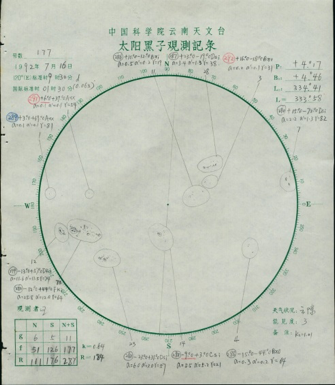
\includegraphics[width=7cm]{fig01.png}
  \caption{太阳黑子手绘图像原图}
\end{figure}

\section{Lab色彩空间}
上面已经提到,太阳黑子手绘图的印刷和手绘部分的颜色都较为集中,但是亮度可能有较大的差别。为了准确的对印刷部分进行识别,我们需要找到一种方法来排除亮度的影响,同时能够准确的度量颜色之间的差异。要达到这些目的,需要选择合适的色彩空间。在这里,我们选择了Lab色彩空间而不是使用最广泛的RGB色彩空间。理由如下:RGB色彩空间是通过R、G、B三基色不同程度的迭加来产生不同的色彩,其中三个色彩分量之间相互影响,任意一个分量的变化引起亮度和色彩的同时变化,而且其色彩分布是不均匀的。显然,RGB色彩空间对本问题并不合适,而Lab空间能够满足我们的要求,下面对Lab空间给出一个简单的介绍。

1976年,国际照明委员会(International Commission on Illumination)为了近似人类视觉,设计出了由$L^*$、$a^*$、$b^*$三个基本坐标组成的CIE L*a*b*(CIELAB)色彩模型,后文省略*,简写为Lab色彩空间。Lab色彩空间属于色彩-对立空间,基于非线性压缩的CIE XYZ色彩空间,使用MacAdam椭圆所描述的色彩差异度量来建立线性化的色彩差异感知,致力于感知均匀性,即在色彩空间中相同的距离对应色彩上相同的差别,弥补了RGB色彩空间色彩分布不均的问题。Lab色彩空间相比其他色彩空间,更接近人眼对色彩的感觉,坐标的亮度信息和色彩信息分开保存,其中维度$L$表示明度,$a$和$b$表示色彩对立维度,通过修改$a$、$b$色彩分量的输出色阶可以达到精确的色彩平衡。在Lab色彩空间中,每个具有$L$、$a$、$b$三个分量的色彩都可以近似为三维空间中的一个点,任何两个色彩的相对感知差别,可以通过计算他们之间的欧几里得距离得到,通常用$\Delta E_{ab}^*$来表示。假设Lab色彩空间中的两个色彩为$(L_1,a_1,b_1)$和$(L_2,a_2,b_2)$:
\begin{equation}
  \Delta E_{ab}^* = \sqrt{(L_2 - L_1)^2 + (a_2 - a_1)^2 + (b_2 - b_1)^2}.
\end{equation}

实现RGB色彩空间到Lab色彩空间的转换需要先将RGB色彩空间转换为XYZ色彩空间,假设r,g,b为三个像素通道,取值范围均为$[0,255]$,转换公式如下所示:
\begin{equation}
  \left\{
    \begin{gathered}
      R_{srgb} = g(\frac{r}{255.0}) \\
      G_{srgb} = g(\frac{g}{255.0}) \\
      B_{srgb} = g(\frac{b}{255.0})
    \end{gathered}
  \right.
\end{equation}
其中$R_{srgb},G_{srgb},B_{srgb} \in [0,1]$.
\begin{equation}
  \begin{pmatrix}
    X \\ Y \\ Z
  \end{pmatrix} =
  \begin{pmatrix}
    0.4124 & 0.3576 & 0.1805 \\
    0.2126 & 0.7152 & 0.0722 \\
    0.0193 & 0.1192 & 0.9505
  \end{pmatrix}
  \begin{pmatrix}
    g(R_{srgb}) \\
    g(G_{srgb}) \\
    g(B_{srgb})
  \end{pmatrix}
\end{equation}
其中
\begin{equation}
  g(k) =
  \begin{dcases}
    \frac{k}{12.92}, & k \leq 0.04045 \\
    {\left(\frac{k+0.055}{1.055}\right)}^{2.4}, & k > 0.04
  \end{dcases}
\end{equation}
式中$g(k)$函数用来对图像进行非线性色调的编辑,目的是提高图像对比度,函数不唯一。

然后,将XYZ色彩空间转换为Lab色彩空间,转换公式如下所示:
\begin{equation}
  \left\{
    \begin{lgathered}
      L = 116 f(Y/Y_n) - 16 \\
      a = 500[f(X/X_n) - f(Y/X_n)] \\
      b = 200[f(Y/Y_n) - f(Z/Z_n)]
    \end{lgathered}
  \right.
\end{equation}
式中$L$、$a$、$b$是最终的Lab色彩空间三个通道的值;X、Y、Z是RGB色彩空间转换为XYZ色彩空间后计算出来的值。Xn、Yn、Zn一般默认是95.047、100.0、108.883。

\section{K-means聚类与最近质心分类器}

聚类的基本思想是通过数据自身的特点,将给定的数据集合自动的划分为若干个由相似的数据点组成的子集。聚类的方法很多,可以分为划分法、层次法、基于密度的方法、基于网格的方法、基于模型的方法等。K-means算法\cite{蒋帅2010k,吴晓蓉2008k}是一种无监督学习的划分法,是很典型的基于距离的聚类算法,即认为两个对象的距离越近,其相似度就越大。该算法思想简便,用于图像分割具有快速、直观、易于实现的优点,容易实现对大规模数据的聚类。

假设提取到的原始数据的集合为$D = \{\vb*{x}_1, \vb*{x}_2, \ldots, \vb*{x}_n\}$,并且每个$\vb*{x}_j$为$d$维的向量,在给定分类组数$k(k\leq n)$的条件下,将原始数据划分成个$k$个子集$\vb*{S} = \{S_1, S_2, \ldots, S_k\}$,$\vb*{\mu}_i$为样本$S_i$的中心点。K-means聚类的目的就是找到一个划分$\vb*{S}$,使其类内平方和最小,即每个点到其所属类的中心点的距离的平方和最小。写成数学表达式,即求解下述最优化问题:
\begin{equation}
  \argmin_{\vb*{S}} \sum_{i = 1}^k \sum_{\vb*{x} \in S_i} \norm{\vb*{x} - \vb*{\mu}_i}^2.
\end{equation}
对上述目标函数的求解一般采用迭代法,具体步骤如下:
\begin{enumerate}
\item 初始化聚类中心点,即随机选取$k$个点$\vb*{\mu}_1^{(1)}, \vb*{\mu}_2^{(1)}, \ldots, \vb*{\mu}_k^{(1)}$, 作为聚类中心点。
\item 对剩余的每一个点$\vb*{x}_j$计算其到中心点的距离,并把它归到距离最近的中心点的类,计算准则为:
  \begin{equation}
    S_i^{(t)} = \left\{ \vb*{x}_p : \norm{\vb*{x}_p - \vb*{\mu}_i^{(t)}}^2 \leq \norm{\vb*{x}_p - \vb*{\mu}_j^{(t)}}^2 , 1 \leq j \leq k \right\}, \quad \forall i.
  \end{equation}
  其中,$S_i^{(t)}$表示第$t$次迭代后属于第$i$类的点的集合,$\vb*{\mu}_i^{(t)}$为第$t$次迭代前的中心点。
\item 根据聚类结果,重新计算已经得到的各类的中心点,计算方法为取各类的所有点的算术平均值:
  \begin{equation}
    \vb*{\mu}_i^{(t+1)} = \frac{1}{|S_i^{(t)}|} \sum_{\vb*{x}_j \in S_i^{(t)}} \vb*{x}_j
  \end{equation}
\item 迭代2--3步,直至$\vb*{\mu}_i^{(t)} = \vb*{\mu}_i^{(t+1)}$或者$|\vb*{\mu}_i^{(t+1)} - \vb*{\mu}_i^{(t)}| < \delta$,$\delta$为指定阈值,算法结束。
\end{enumerate}

若已对一部分数据进行了K-means聚类,当需要对新的数据进行分类的时候,可不必重新聚类而直接用最近质心分类器对其进行分类。在机器学习中,最近质心分类器是一种分类模型,它将待分类数据归为与其最近的样本分类质心所在的类。具体过程如下:给定训练样本$\{(\vb*{x}_1,y_1), \ldots, (\vb*{x}_n,y_n)\}$其中类标签$y_i \in \vb{Y}$, 计算各个类的质心
\begin{equation}
\vb*{\mu}_l = \frac{1}{|C_l|} \sum_{i\in C_l} \vb*{x}_i,
\end{equation}
其中$C_l$为属于类$l\in \vb{Y}$的样本的下标的集合。待分类数据$\vb*{x}$的预测函数为
\begin{equation}
  \hat{y} = \argmin_{l\in \vb{Y}} \norm{\vb*{\mu}_l - \vb*{x}}.
\end{equation}

对于大量需要分类的数据,可以结合K-means聚类和最近质心分类法,以便于减少计算时间。首先,选取部分数据进行K-means聚类,将这部分已分类的数据作为样本数据。然后利用最近质心分类器对剩下的数据进行分类。对于本文所讨论大批量太阳黑子手绘图的背景提取问题,即采用此方法处理,具体结果见下节。

% \subsection{Lab色彩空间中a、b分量的K-means聚类}
% 传统的太阳黑子手绘观测记录是纸介质的,在保存过程中受到外界温度、湿度等条件影响,纸张本身会受潮产生斑点及变形,会降低数字扫描图像质量,导致黑子图像噪点较多、背景斑驳等。在RGB色彩空间直接进行K-means聚类效果不理想。但是黑子手绘图像中印刷部分和手绘部分采用不同色彩记录,为只针对色彩的聚类提供了可能性。这里我们抛开明度L的影响,对a、b色彩分量,进行K-means聚类。
% 每个具有a、b两个分量的色彩都可以近似为二维空间中的一个点,任何两个色彩的相对感知差别可以用他们的Euclidean distance(欧几里得距离)表示。对a、b色彩分量进行K-means聚类,可以看作在以a、b色彩分量值为坐标轴的二维空间中,对所有色彩点之间距离的聚类。那么,对目标函数的求解问题,可以利用函数求极值的方法得到迭代运算的调整规则,并对目标函数进行优化,具体过程如下:

% \subsection{寻找判别函数}
% 对于我们研究的问题,我们只需要将所有色彩点分为印刷部分和非印刷部分这两类,利用2.2中所介绍的K-means聚类方法,我们可以得到这两类的质心,根据7式所给出的判断准则,对于色彩空间中的任意一点,把它归到最近的质心的类。对于两类的情况,我们可以找到一条分界线,位于分界线两侧的色彩点与同侧的质心属于同一类。显然,位于分界线上的色彩点与两个质心的距离相等,这条分界线就是这两个质心的连线的中垂线。对于质心 , ,其中垂线方程为 

\section{实验与结论}

首先,按照第2节中的方法将所有的太阳黑子手绘图转换到Lab色彩空间。由于我们仅对像素点的颜色感兴趣,对亮度不感兴趣,所以我们只考虑Lab色彩空间的$a$和$b$分量。选取一张手绘图,其像素点在$a$,$b$分量上的等高线对数分布图,如图\ref{abDistribute} 所示。

\begin{figure}[H]
  \centering
  \includegraphics[width=8cm]{abDistribute.jpg}
  \caption{太阳黑子手绘图像素的$a$,$b$分量对数分布图}\label{abDistribute}
\end{figure}

在所有的太阳黑子手绘图中进行随机抽样,对所有样本的像素的$a$,$b$分量按照第2节中的方法进行两类K-means聚类,即令$k = 2$。聚类的结果见图\ref{clusterResult}--\ref{directCluster_c}。其中,图\ref{clusterResult} 为$a,b$平面的聚类结果图;图\ref{directCluster_a} 为局部原始图像;图\ref{directCluster_b} 为聚类后分离出来的背景图,其对应图\ref{clusterResult} 中左上部分的那一类;图\ref{directCluster_c} 为聚类后分离的手绘图,其对应图\ref{clusterResult} 中右下部分的那一类。从图中的结果表明,此方法能够很好的对背景进行识别与提取。

\begin{figure}[H]
  \centering
  \includegraphics[width=8cm]{clusterResult.png}
  \caption{$a, b$平面的聚类结果图}
  \label{clusterResult}
\end{figure}

\begin{figure}[H]
  \centering
  \begin{minipage}{5cm}
    \centering
    \includegraphics[width=5cm]{directCluster_a.png}
    \caption{局部原始图像}
    \label{directCluster_a}
  \end{minipage}
  \hspace{0.2cm}%
  \begin{minipage}{5cm}
    \centering
    \includegraphics[width=5cm]{directCluster_b.png}
    \caption{局部背景图像}
    \label{directCluster_b}
  \end{minipage}
  \hspace{0.2cm}%
  \begin{minipage}{5cm}
    \centering
    \includegraphics[width=5cm]{directCluster_c.png}
    \caption{局部手绘部分图像}
    \label{directCluster_c}
  \end{minipage}
\end{figure}

对于大批量手绘图的背景提取,为加快计算速度,我们采用第4节中介绍的方法,即结合K-means聚类与最近质心分类器对剩余的手绘图进行背景提取。图\ref{compare_1}--\ref{compare_3}为直接聚类和最近质心分类器的背景提取效果对比图。从图中可以发现,才用最近质心分类器的背景提取效果与直接聚类的效果相差无几。

\begin{figure}[H]
  \centering
  \begin{minipage}{5cm}
    \centering
    \includegraphics[width=5cm]{compare_1.png}
    \caption{局部原始图像}
    \label{compare_1}
  \end{minipage}
  \hspace{0.2cm}%
  \begin{minipage}{5cm}
    \centering
    \includegraphics[width=5cm]{compare_2.png}
    \caption{直接聚类提取的背景}
    \label{compare_2}
  \end{minipage}
  \hspace{0.2cm}%
  \begin{minipage}{5cm}
    \centering
    \includegraphics[width=5cm]{compare_3.png}
    \caption{最近质心分类器提取的背景}
    \label{compare_3}
  \end{minipage}
\end{figure}


% \subsection{基于判断准则的背景提取}
% 对所有的太阳黑子手绘图进行随机抽样,转换到Lab空间后,对样本总体的a,b分量进行K-means聚类,聚类结果图如图3所示。最后直接利用聚类得到的分割准则对其他的手绘图进行分割。图4、5分别为印刷与手绘部分整幅图像分割结果。

% \subsection{Lab色彩空间和RGB色彩空间聚类划分对比分析}

% \subsection{聚类和判断准则划分对比分析}

\section{结语}

本文提出了一种基于Lab色彩空间的太阳黑子手绘图分割方法,该方法不考虑明度对图像分割的影响,仅通过a、b色彩对印刷部分和手绘部分进行分割,达到了较理想的效果。通过K均值聚类将印刷部分分离出来,设置印刷部分为白色,显示的图像即为手绘部分。最后根据K均值聚类寻找判断准则来替代该聚类,达到同样效果的前提下,很大程度上节省了批量处理的时间。实验表明,该方法能准确的分离太阳黑子手绘图的印刷部分和手绘部分。本文提出的算法也有不足之处,比如由RGB色彩空间转换到Lab空间较耗时。


\bibliographystyle{unsrt}

\bibliography{ref}

\end{document}

%%% Local Variables:
%%% mode: latex
%%% TeX-master: t
%%% End:
